\section{Développement de la schématique} \label{sec:Dev-Schematique}
Dans cette section, nous décrirons la phase principale du développement ainsi que la démarche suivie pour élaborer le schéma électronique du projet.

\subsection{Blocs développés} \label{ssec:Dev-blocs}
Pour faciliter le développement et la lecture du schéma, il est judicieux de diviser le système en plusieurs blocs. Une structure a ainsi été définie, divisant le circuit en trois blocs principaux : \fbox{\hyperref[ssec:Dev-MCU]{\textbf{Microcontrôleur \ref{ssec:Dev-MCU}}}}, \fbox{\hyperref[ssec:Dev-Devices]{\textbf{Périphériques \ref{ssec:Dev-Devices}}}} et \fbox{\hyperref[ssec:Dev-Power]{\textbf{Puissance \ref{ssec:Dev-Power}}}}.



\subsection{Microcontrôleur} \label{ssec:Dev-MCU}
\clearpage

\begin{figure}[h]
	\centering
	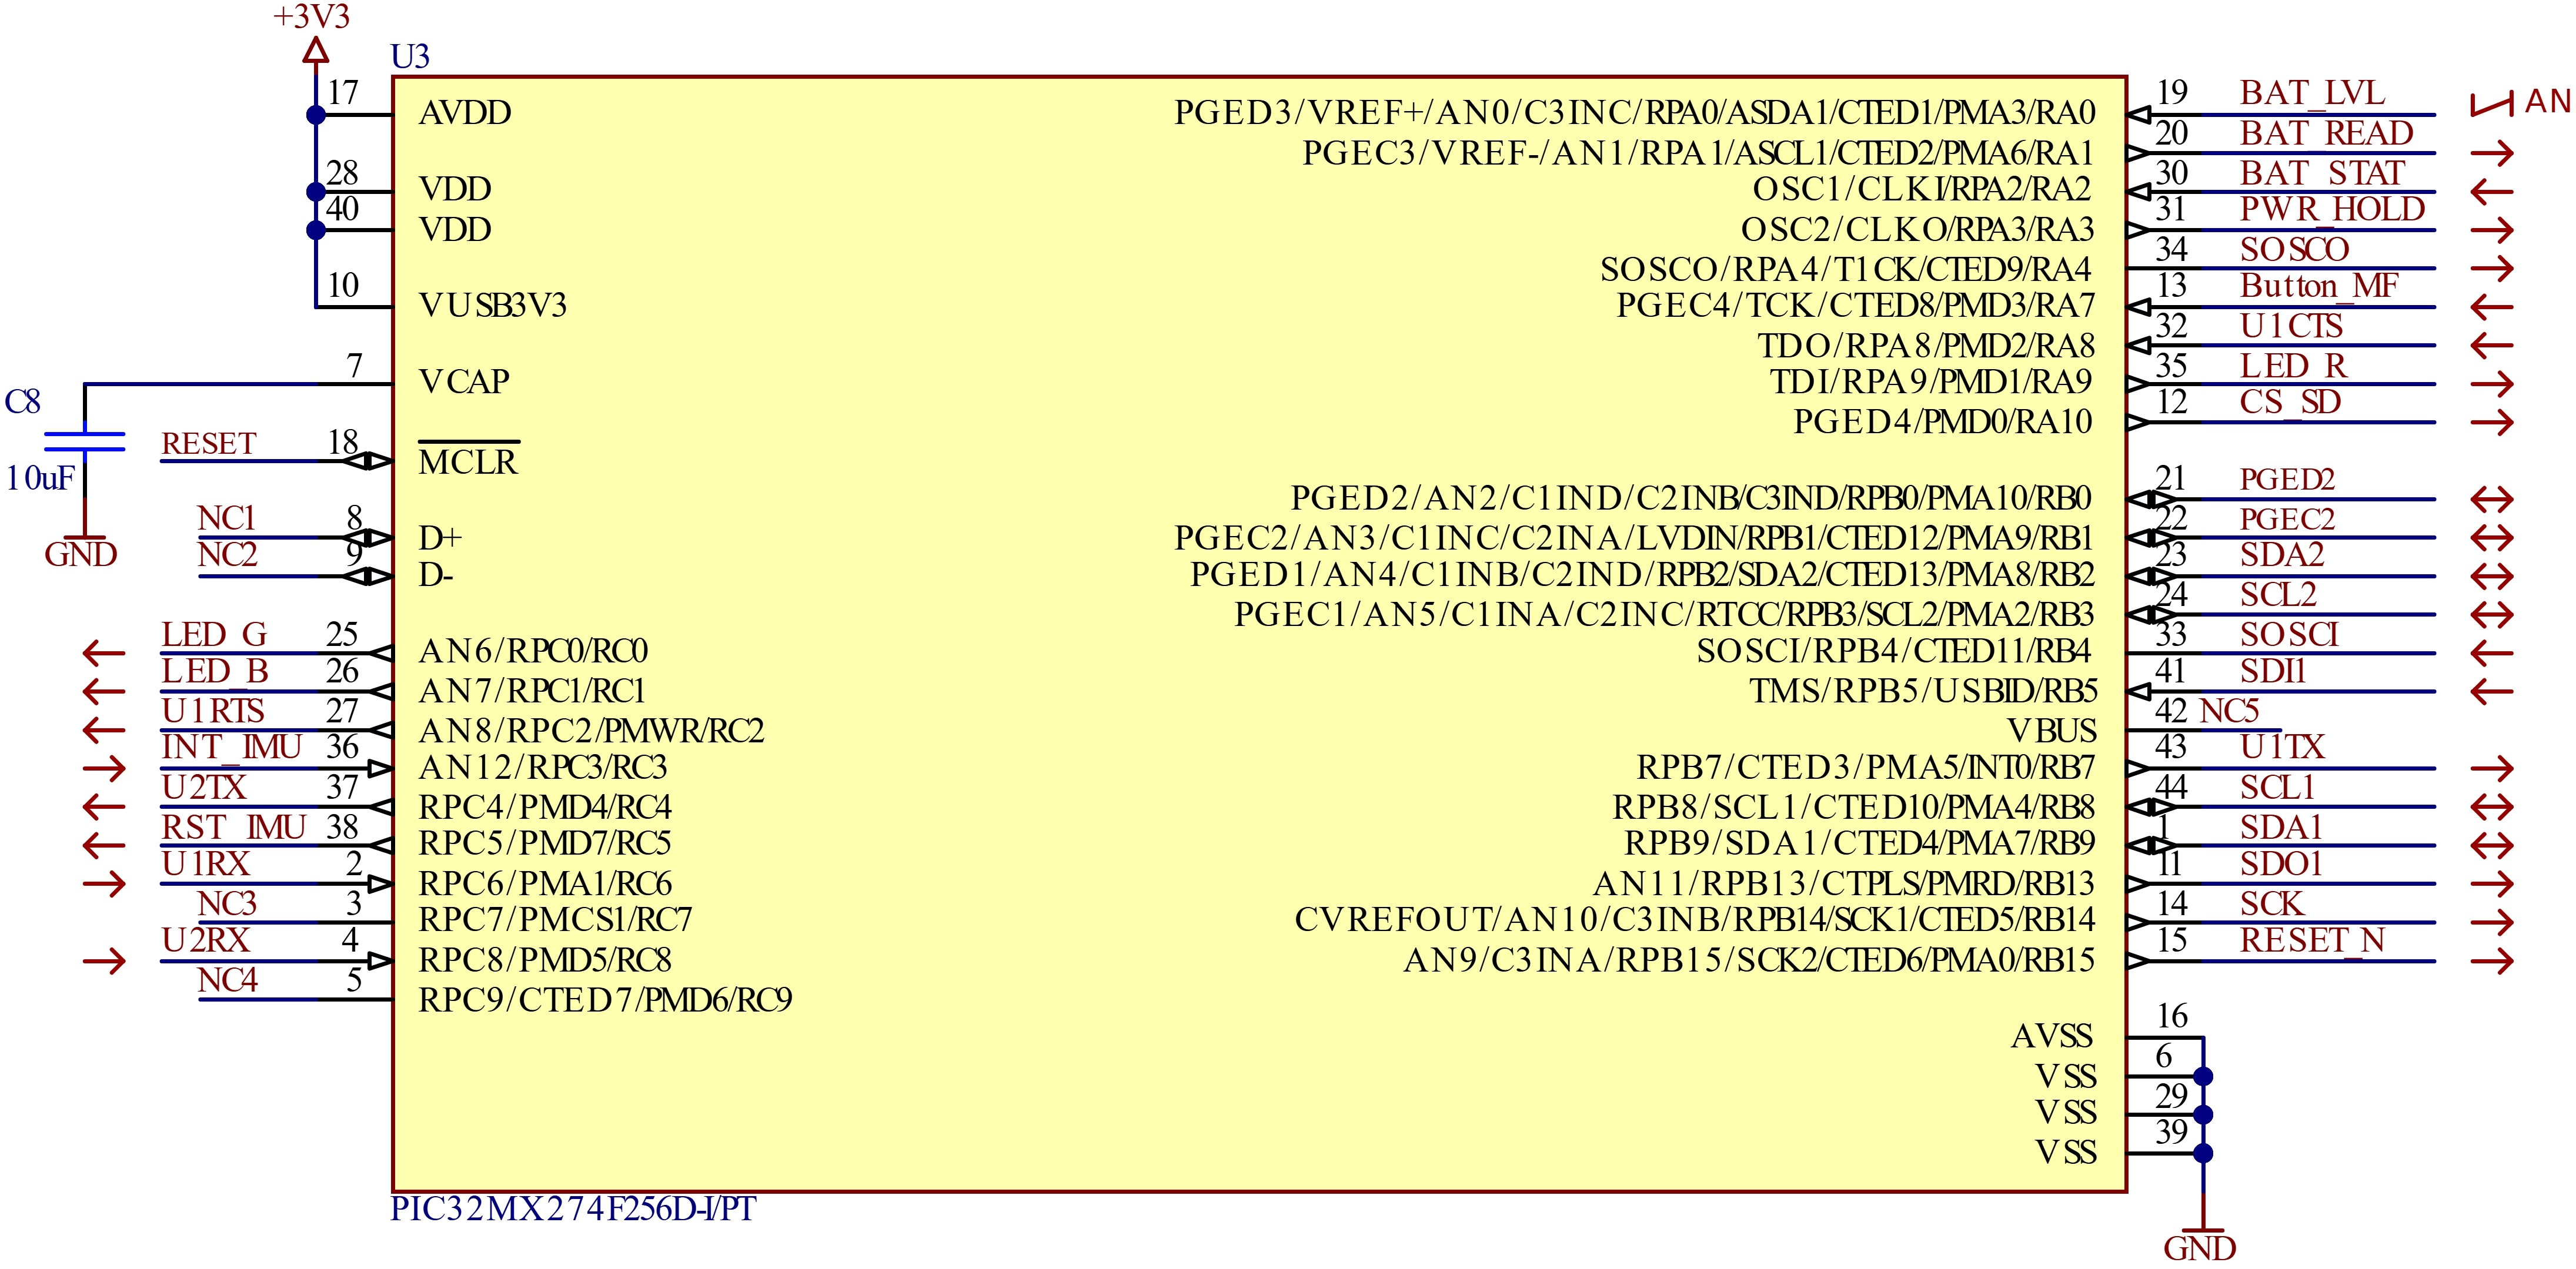
\includegraphics[width=1\linewidth]{../figures/etude/sch/MCU}
	\caption{Connexions du microcontrôleur}
	\label{fig:mcu}
\end{figure}

\subsection{Périphériques} \label{ssec:Dev-Devices}

\subsection{Puissance} \label{ssec:Dev-Power}

\subsection{Dimensionnements} \label{ssec:Dev-Dimensionnements}

\subsubsection{Bus de communications} \label{sssec:Dev-BusComm}

\subsubsection{Interface} \label{sssec:Interface}

\subsubsection{Périphériques} \label{sssec:Peripheriques}

\subsubsection{Chargeur de batterie} \label{sssec:Chargeur-bat}

\subsubsection{Adaptation mécanique} \label{sssec:Adaptation-mech}

\subsection{Synthèse et perspectives de l'étude} \label{ssec:Synth-etude}